The Belle II detector employs a layered, cylindrical design where different subsystems work together to provide comprehensive particle detection and measurement capabilities.
Each component is optimized to handle the challenging environment of high luminosity $e^+e^-$ collisions while maintaining high resolution and efficiency across a wide range of particle momenta.

The following paragraphs provide an overview of the most important detector components and their functions, starting from the innermost layers and moving outward.
For a schematic representation of the Belle II detector and its main components, see Figure \ref{fig:belle2-schematics}.

\paragraph{Interaction Point and Beam Pipe}
The electron and positron beams collide at the interaction point (IP), located at the center of the Belle II detector.
By convention, particle positions and momenta are described in a coordinate system where the z-axis is aligned with the solenoid's central axis and points in the direction of the electron beam, and the origin lies in the interaction point (Fig.\ \ref{fig:belle2-schematics}, right).

The beam pipe, which also coincides with the z-axis, contains the colliding beams and is maintained under high vacuum conditions to minimize beam-gas interactions that produce unwanted background events.
Near the interaction point, it is constructed from beryllium, with a cylindrical inner radius of \qty{10}{\milli\meter}.
The element beryllium was chosen for its favorable properties: it provides adequate vacuum containment while maintaining minimal material thickness.
This design consideration is important because particles produced in collisions must traverse the beam pipe material, and excessive thickness would degrade the precision of vertex and momentum measurements.
When particles pass through the material, they experience energy loss through ionization and multiple scattering processes, effects that directly impact particle reconstruction accuracy and must be properly accounted for in both the tracking algorithms and subsequent physics analyses.

\paragraph{Vertex Detector System}
The vertex detector system (VXD) consists of two layers of pixel detectors (PXD) and four layers of silicon strip detectors (SVD) arranged around the beam pipe.
The pixel detectors form the innermost layers and provide precise position measurements, while the strip detectors constitute the outer layers.
When charged particles traverse these silicon sensors, they deposit energy that generates electrical signals.
This system measures particle trajectories close to the interaction point, enabling accurate reconstruction of particle production and decay vertices.

\paragraph{Central Drift Chamber}
The Central Drift Chamber (CDC) is a cylindrical gas-filled detector that surrounds the VXD.
When charged particles traverse the gas volume, they ionize atoms along their trajectory.
The freed electrons subsequently drift toward sense wires under an applied electric field, creating electron avalanches that produce measurable signals upon arrival.
Using geometric triangulation, particles' positions at the time of initial ionization can be reconstructed from the measured signal times of individual wires and the known electron drift velocity.
This enables precise reconstruction of charged particle trajectories, from which particle momenta can be determined via their curvature in the magnetic field.

\paragraph{Particle Identification Systems}
Belle II employs two distinct Cherenkov detectors for particle identification in different detector regions.
They both exploit the fact that charged particles with identical momentum but different masses travel at different velocities, producing distinct Cherenkov light signatures that allow reliable particle type determination.

The barrel region, which covers the central cylindrical area around the interaction point, houses the Time-of-Propagation (TOP) counter.
This detector records both the positions and the arrival times of Cherenkov photons produced by charged particles traversing quartz radiator bars.
Different particle species produce Cherenkov photons at characteristic angles depending on their velocity, resulting in distinct patterns of photon arrival times and positions at the detector.

The forward endcap region, covering the area along the beam direction where particles are boosted due to the asymmetric beam energies, contains the Aerogel Ring Imaging Cherenkov Detector (ARICH).
This system uses aerogel as the radiating medium and detects the characteristic ring patterns formed by Cherenkov photons, with the ring radii depending on the particles' velocities.

Both detectors achieve particle identification by combining their respective Cherenkov signatures with momentum measurements from the CDC, enabling mass determination through the relationship between momentum, velocity, and mass.

\paragraph{Electromagnetic Calorimeter}
The electromagnetic calorimeter (ECL) is made up of thousands of thallium-doped cesium iodide crystals arranged in layers surrounding the interaction region.
When high-energy photons or electrons enter the crystals, they initiate electromagnetic showers through repeated bremsstrahlung and pair production processes.
These showers generate scintillation light within the crystals, with the intensity of the emitted light being proportional to the energy deposited by the particle, enabling the measurement of incident particles' energies.

\paragraph{Muon and K-long Detection System}
The outermost detector component is the K-long and muon detection system (KLM), which consists of alternating iron plates and active detector elements.
K-long particles (neutral kaons) interact hadronically within the iron absorbers and produce detectable particle showers.
Muons are identified primarily by their ability to penetrate through all inner detector layers and the iron absorber with minimal interaction, unlike most other charged particles.
As they pass through the active KLM elements, they deposit energy via ionization, allowing them to be traced through the entire detector, and enabling their identification.

Identification of muons is crucial for many important B-meson decays, and the KLM also facilitates the detection of neutral kaons that would otherwise remain undetected.

\paragraph{Superconducting Solenoid}
A superconducting magnet surrounds most of the detector components, creating a uniform magnetic field throughout the tracking region.
This magnetic field causes charged particles to follow curved trajectories, with the radius of curvature directly related to the particle's momentum and charge.
The magnetic field is essential for precise momentum measurements and charge identification of particles.
The iron return yoke that contains and shapes the magnetic field additionally serves as absorber material for the KLM.

\begin{figure}[htbp]
  \centering
  \begin{minipage}[c]{0.5\textwidth}
    \centering
    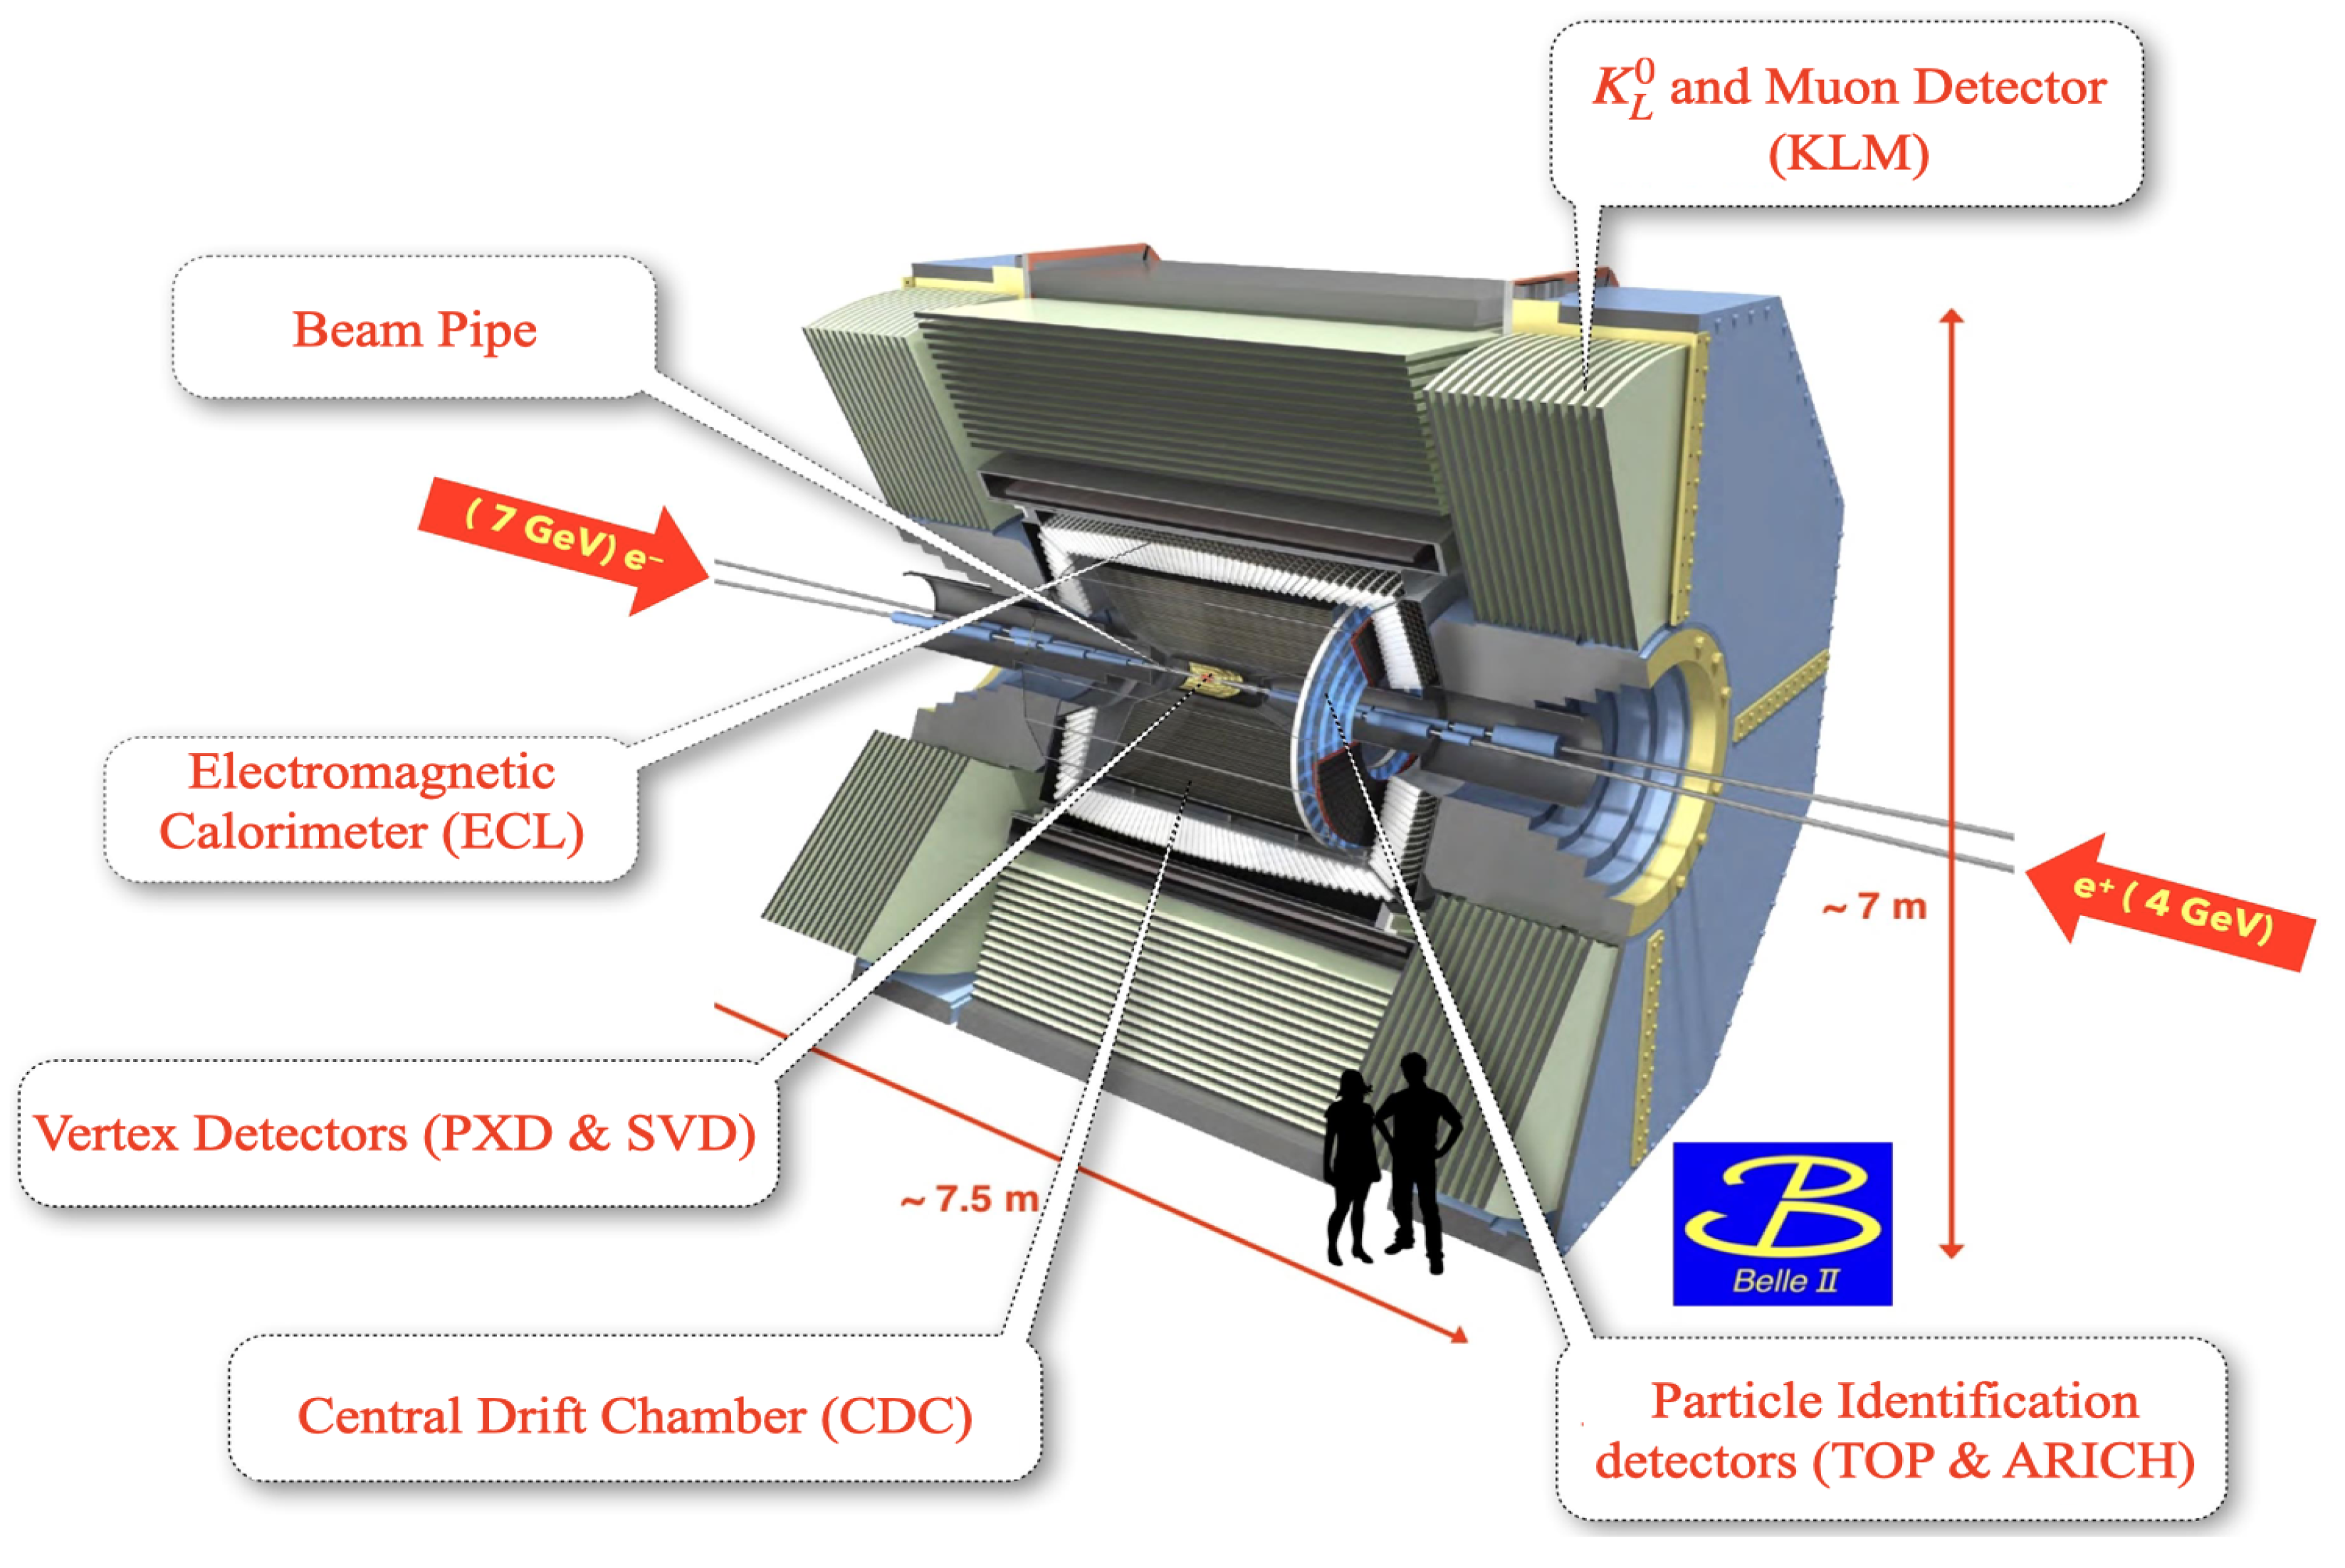
\includegraphics[width=\linewidth]{static/belle2-components.png}
  \end{minipage}%
  \vrule%
  \begin{minipage}[c]{0.5\textwidth}
    \centering
    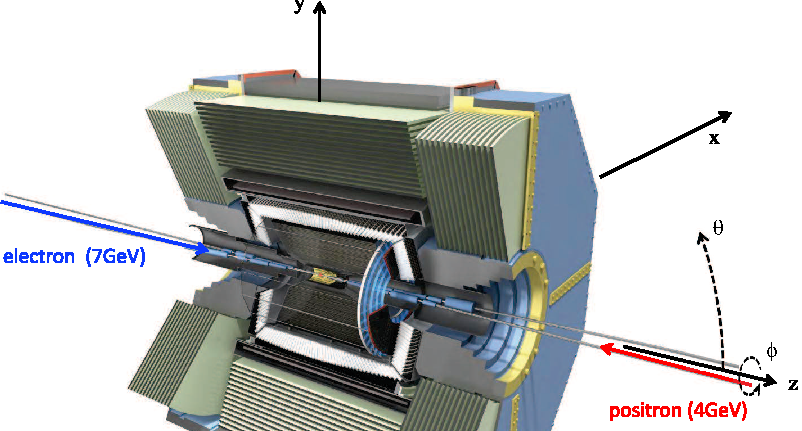
\includegraphics[width=\linewidth]{static/basf2-coordinate-system.pdf}
  \end{minipage}
  \caption{%
    \\\emph{Left:} Cross-sectional view of the Belle II detector with labeled subsystems and beam configuration \cite{belle2-components}\\
    \emph{Right:} Belle II experiment coordinate system (convention used in the Belle II software)  \cite{belle2-coordinates}
  }
  \label{fig:belle2-schematics}
\end{figure}